\documentclass{article}
\usepackage{appendix}
\usepackage{multicol}
\usepackage{leftidx}
\usepackage{ragged2e}
\usepackage{hyperref}
\usepackage{amsthm}
\usepackage{bbold}
\usepackage{subfiles}
\usepackage{mathtools}
\usepackage{units}
\usepackage{graphicx}
\usepackage{float}
\usepackage{subcaption}
\usepackage{commath}
\usepackage{tcolorbox, varwidth} % Boxes
\usepackage{amsthm} % For the proof environment

\tcbuselibrary{breakable}
\tcbuselibrary{theorems}
\tcbuselibrary{skins}

% Colours
\definecolor{TheoremColor}{RGB}{0,0,0} % Green
\definecolor{DefColor}{RGB}{45, 52, 2} % Blue
\definecolor{CorollaryColor}{RGB}{158, 80, 143} % Purple
\definecolor{ExampleColor}{RGB}{226,135,67} % Orange
\definecolor{ProofColor}{RGB}{0,177,160} % Aqua
\definecolor{FactColor}{RGB}{124,23,12} % Aqua


\title{Appunti sulla Computazione Quantistica}
\author{Victor Lopata}
\date{July 2024}



\newpage

\begin{document}
    \maketitle
    \tableofcontents
    \newpage
	% Theorem
\newtcbtheorem[number within = section]{theorem}{Theorem}%
{enhanced,frame empty,interior empty,colframe=TheoremColor!50!white,
	coltitle=TheoremColor!50!black,fonttitle=\bfseries,colbacktitle=TheoremColor!15!white,
	borderline={0.5mm}{0mm}{TheoremColor!15!white},
	borderline={0.5mm}{0mm}{TheoremColor!50!white},
	attach boxed title to top left={yshift=-2mm, xshift=3mm},
	boxed title style={boxrule=0.4pt},varwidth boxed title}{theo}

% Definition
\newtcbtheorem[number within = section]{definition}{Definition}%
{enhanced,frame empty,interior empty,colframe=DefColor!50!white,
	coltitle=DefColor!50!black,fonttitle=\bfseries,colbacktitle=DefColor!15!white,
	borderline={0.5mm}{0mm}{DefColor!15!white},
	borderline={0.5mm}{0mm}{DefColor!50!white},
	attach boxed title to top left={yshift=-2mm, xshift=3mm},
	boxed title style={boxrule=0.4pt},varwidth boxed title}{defo}

% Corollary
\newtcbtheorem[number within = section]{corollary}{Corollary}%
{enhanced,frame empty,interior empty,colframe=CorollaryColor!50!white,
	coltitle=CorollaryColor!50!black,fonttitle=\bfseries,colbacktitle=CorollaryColor!15!white,
	borderline={0.5mm}{0mm}{CorollaryColor!15!white},
	borderline={0.5mm}{0mm}{CorollaryColor!50!white},
	attach boxed title to top left={yshift=-2mm, xshift=3mm},
	boxed title style={boxrule=0.4pt},varwidth boxed title}{defo}
 
% Osservazione
\newtcbtheorem[number within = section]{oss}{Observation}%
{enhanced,frame empty,interior empty,colframe=CorollaryColor!50!white,
	coltitle=CorollaryColor!50!black,fonttitle=\bfseries,colbacktitle=CorollaryColor!15!white,
	borderline={0.5mm}{0mm}{CorollaryColor!15!white},
	borderline={0.5mm}{0mm}{CorollaryColor!50!white},
	attach boxed title to top left={yshift=-2mm, xshift=3mm},
	boxed title style={boxrule=0.4pt},varwidth boxed title}{defo}
 
% Example
\newtcbtheorem[number within = section]{example}{Example}%
{enhanced,frame empty,interior empty,colframe=ExampleColor!50!white,
	coltitle=ExampleColor!50!black,fonttitle=\bfseries,colbacktitle=ExampleColor!15!white,
	borderline={0.5mm}{0mm}{ExampleColor!15!white},
	borderline={0.5mm}{0mm}{ExampleColor!50!white},
	attach boxed title to top left={yshift=-2mm, xshift=3mm},
	boxed title style={boxrule=0.4pt},varwidth boxed title}{defo}

% Proof
\tcolorboxenvironment{proof}{% `proof' from `amsthm'
	blanker,breakable,left=5mm,
	before skip=10pt,after skip=10pt,
	borderline west={1mm}{0pt}{ProofColor!50!white}}

% Fact
\newtcbtheorem[number within = section]{fact}{Fact}%
{enhanced,frame empty,interior empty,colframe=ExampleColor!50!white,
	coltitle=ExampleColor!50!black,fonttitle=\bfseries,colbacktitle=ExampleColor!15!white,
	borderline={0.5mm}{0mm}{FactColor!15!white},
	borderline={0.5mm}{0mm}{FactColor!50!white},
	attach boxed title to top left={yshift=-2mm, xshift=3mm},
	boxed title style={boxrule=0.4pt},varwidth boxed title}{facto}
\section{Nozioni Matematiche}
\subsection{Strutture algebriche}
\begin{definition}{Struttura Algebrica}{}
    Definiamo come \textbf{struttura algebrica} un insieme munito di una o più operazioni. Spesso viene indicato con la notazione $(A, m)$, dove $A$ è l'insieme ed $m$ è l'operazione.
\end{definition}

\begin{definition}{Principali strutture algebriche}{}
    Sia $(A,m)$ una struttura algebrica, dove $A$ è l'insieme ed $m$ è un'operazione binaria chiusa sull'insieme. 
    Tale struttura può essere definita come:
    \begin{itemize}
        \item \textbf{Semigruppo}: se $m$ è \underline{associativa}.
        \item \textbf{Monoide}: se $m$ è \underline{associativa} e munita dell'\underline{elemento neutro}.
        \item \textbf{Gruppo}: se $m$ è \underline{associativa}, munita dell'\underline{elemento neutro} e dell'\underline{elemento inverso}.
        \item \textbf{Gruppo abeliano}: se $m$ è \underline{associativa}, munita dell'\underline{elemento} \underline{neutro} e dell'\underline{elemento inverso} ed è \underline{commutativa}.
    \end{itemize}
\end{definition}

\begin{definition}{Anello}{}
    Sia $(A,+,\cdot)$ una struttura algebrica. Possiamo definirla come \textbf{anello} se:
    \begin{itemize}
        \item $(A,+)$ è un \textbf{gruppo abeliano}.
        \item $(A,\cdot)$ è un \textbf{semigruppo}.
        \item La moltiplicazione è distributiva rispetto alla somma:
        \begin{equation*}
            \begin{split}
                a \cdot (b + c) = (a \cdot b) + (a \cdot c) \\
                (a + b) \cdot c= (a \cdot c) + (b \cdot c)   
            \end{split}
        \end{equation*}
    \end{itemize}
    Possiamo definirlo anche come \textbf{anello commutativo} se $(A,\cdot)$ è munita della commutatività.
\end{definition}
\begin{fact}{}{}
    Sia $(A,+,\cdot)$ un anello. Allora:
    \begin{equation*}
        \forall x,y\in A \quad (xy)^{-1} = y^{-1}x^{-1}
    \end{equation*}
\end{fact}
\begin{definition}{Campo}{}
    Sia $(K,+,\cdot)$ una struttura algebrica. Possiamo deifinirla come \textbf{campo} se:
    \begin{itemize}
        \item $(K,+,\cdot)$ è un \textbf{anello commutativo}.
        \item $(K \backslash \{0\},\cdot)$ è un \textbf{gruppo abeliano}.
    \end{itemize}
\end{definition}

\subsection{Numeri complessi}
\subsection{Spazi Vettoriali}
\begin{definition}{Norma Euclidiana}{}
    Sia $v$ un vettore avente numeri complessi come entrate:
    \begin{equation*}
        v = \left(
        \begin{array}{c}
             \alpha_1  \\
             \vdots \\
            \alpha_n   
        \end{array}\right)
    \end{equation*}
    Definiamo la sua \textbf{norma Euclidiana} come:
    \begin{equation}
        \Vert v \Vert = \sqrt{\sum_{k=1}^{n} |{\alpha_k}^2|}
    \end{equation}
\end{definition}
\subsection{Matrici}
\begin{definition}{Trasposta di una matrice}{}
    Sia $A$ una matrice. Definiamo come \textbf{matrice trasposta} di $A$, rappresentata dal simbolo $A^{\mathrm{T}}$, come la matrice avente il cui generico elemento con indici $(i,j)$ è l'elemento con indice $(j,i)$ della matrice originaria.
    In altre parole, la matrice trasposta di una matrice è la matrice ottenuta scambiandone le righe con le colonne.
\end{definition}
\begin{example}{}{}
\begin{itemize}
    \item $A = \left(\begin{array}{ccc}
        2 & 1 & 4 \\
        0 & 0 & 3
    \end{array}\right) \quad A^{\mathrm{T}} = \left(\begin{array}       {cc}
        2 & 0 \\
        1 & 0 \\
        4 & 3
    \end{array}\right)$
    \item $A = \left(\begin{array}{ccccc}
        1 & 2 & 3 & 4 & 5 \\
        6 & 7 & 8 & 9 & 10 \\
        11 & 12 & 13 & 14 & 15 \\
        16 & 17 & 18 & 19 & 20 
    \end{array}\right) \quad A^{\mathrm{T}} = \left(\begin{array}       {cccc}
        1 & 6 & 11 &  16 \\
        2 & 7 & 12 & 17 \\
        3 & 8 & 13 & 18 \\
        4 & 9 & 14 & 19 \\ 
        5 & 10 & 15 & 20 
    \end{array}\right)$
\end{itemize}
\end{example}
\begin{definition}{Matrice Trasposta Coniugata}{}
    Sia $A$ una matrice avente come entrate valori complessi. Deifiniamo la sua \textbf{matrice trasposta coniugata}, rappresentata dal simbolo $A^{\dagger}$, come la matrice ottenuta effettuando la trasposta e scambiando ogni valore con il suo comlesso coniugato.
\end{definition}
\begin{example}{}{}
    $A = \left(\begin{array}{cc}
        3+9i & 2+i \\
        7-6i & 1-3i
    \end{array}\right) \quad A^{\dagger} = \left(\begin{array}       {cc}
        3-9i & 7+6i \\
        2-i & 1+3i \\
    \end{array}\right)$
\end{example}
\begin{definition}{Matrici Unitarie}{}\label{matUnit}
    Sia $U$ una matrice quadrata complessa. Definiamo $U$ come una \textbf{matrice unitaria} se:
    \begin{equation*}
        U^{\dagger}U = \mathbb{1} = UU^{\dagger}
    \end{equation*}
    dove $U^{\dagger}$ è la matrice trasposta coniugata di $U$ e $\mathbb{1}$ è la matrice identità.
\end{definition}
\begin{fact}{}{}
    Sia $U$ una matrice unitaria. Allora abbiamo che:
    \begin{equation*}
        \Vert Uv \Vert = \Vert v \Vert \quad \forall v \text{ vettore}
    \end{equation*}
\end{fact}
\subsection{Notazione Dirac}
    %\section{Informazione Classica}
Per comprendere al meglio come funziona l'informazione e la computazone quantistica, è bene avere le idee chiare su come funziona quella classica.
\subsection{Sistemi Singoli}
Sia $X$ un sistema fisico che memorizza l'informazione. $X$ può stare in un numero \textbf{finito di stati}. Definiamo anche $\Sigma$ come l'insieme finito degli stati che $X$ può assumere.

\begin{example}{}{}
    Ad esempio possiamo pensare ad $X$ come un bit, quindi $\Sigma = \{0,1\}$.
\end{example}

\begin{definition}{Stato Probabilistico}{}
    Sia $X$ un sistema e $\Sigma$ il suo insieme di stati. Definiamo gli \textbf{stati probabilistici} di $X$ se associamo ad ogni stato una \textbf{probabilità} tale che:
    \begin{itemize}
        \item $0 \leq p(\sigma) \leq 1$ per ogni $\sigma \in \Sigma$
        \item $\sum_{\sigma \in \Sigma} p(\sigma) = 1$
    \end{itemize}
\end{definition}

Possiamo rappresentare gli \textbf{stati probabilistici} come vettori, chiamati anche \textbf{vettori probabilistici}.
\begin{example}{}{}
    Sia $X$ il sistema che rappresenta un bit. Con probabilità $\frac{3}{4}$ $X$ assume lo stato di $0$, con $\frac{1}{4}$ assume $1$. Allora possiamo rappresentare questo stato attraverso il seguente vettore:
    \begin{equation*}
         \left(\begin{array}{c}
             \frac{3}{4}  \\ \\
             \frac{1}{4} 
        \end{array}\right)
    \end{equation*}
    dove la prima entrata corrisponde la probabilità che $X$ assuma lo stato $0$, la seconda entrata corrisponde alla probabilità che $X$ assuma lo stato $1$.

\end{example}

È comodo utilizzare la Dirac Notation (Sezione 1.5) per esprimere uno stato probabilistico.

\begin{definition}{Standard Basis Vectors}{}
    Definiamo come \textbf{Standard Basis Vectors} i vettori che hanno tutte le entrate $0$ eccetto una singola entrata avente $1$. Sono utili per rappresentare gli stati classici.
\end{definition}
In particolare, per il nostro sistema binario, gli standard basis vectors sono $|0\rangle$, corrispondente a 
$\left(\begin{array}{c}
         1  \\
         0
    \end{array}\right)$
e $|1\rangle$, corrispondente a $\left(\begin{array}{c}
         0  \\
         1
    \end{array}\right)$.

\begin{fact}{}{}
    Ogni vettore probabilistico può essere espresso unicamente come una \textbf{combinazione lineare} degli standard basis vectors.
\end{fact}
\begin{example}{}{}
    \begin{equation*}
        \left(\begin{array}{c}
         \frac{3}{4}  \\ \\
         \frac{1}{4}
    \end{array}\right) = \frac{3}{4} |0\rangle +  \frac{1}{4} |1\rangle
    \end{equation*}
\end{example}
\subsubsection{Misurazione di stati probabilistici}
\subsubsection{Operazioni deterministiche}
\subsubsection{Operazioni probablistiche}
\subsubsection{Composizione di operazioni probabilistiche}
\subsection{Sistemi Multipli}
\subsubsection{Stati Classici}
\subsubsection{Stati Probabilistici}
\subsubsection{Misurazione di stati probabilistici}
\subsubsection{Operazioni sugli stati probabilistici}

    \section{Introduzione all'informazione quantistica}
\subsection{Sistemi Singoli}
\begin{definition}{Stato Quantistico}{}
    Definiamo come \textbf{stato quantistico} un \textbf{vettore colonna} tale che:
    \begin{itemize}
        \item Le entrate sono \textbf{numeri complessi}
        \item La somma dei valori assoluti elevati alla seconda deve essere uguale ad $1$.
    \end{itemize}
\end{definition}
Le entrate dei vettori colonna, rappresentate dai numeri complessi, sono chiamati anche \textbf{ampiezza}.
\begin{definition}{Stato Quantistico (definizione alternativa)}{}
    Possiamo definire uno stato quantistico anche come un vettore colonna $v$ che ha come entrate numeri complessi tale che $\Vert v \Vert = 1$.
\end{definition}

\begin{example}{Stati Quantistici}{}
\begin{itemize}
    \item $|0\rangle$
    \item $|1\rangle$
    \item $|+\rangle = \frac{1}{\sqrt{2}}|0\rangle +  \frac{1}{\sqrt{2}}|1\rangle$
    \item $|-\rangle = \frac{1}{\sqrt{2}}|0\rangle -  \frac{1}{\sqrt{2}}|1\rangle$
\end{itemize}
\end{example}
Stati quantistici che non hanno una particolare denominazione vengono indicate con le lettere $\psi$ o $\phi$. Ad esempio
\begin{equation*}
    |\psi\rangle = \frac{1 + 2i}{3}|0\rangle -  \frac{2}{3}|1\rangle
\end{equation*}
\subsubsection{Misurazione di stati quantistici}
\subsubsection{Operazioni Unitarie}
Le operazioni che si possono applicare sugli stati quantistici sono rappresentate dalle \textbf{matrici unitarie} (Definizione \ref{matUnit}).
\begin{oss}{}{}
    Se $v$ è uno stato quantistico, allora anche $Uv$ è uno stato quantistico.
\end{oss}
Vediamo alcune delle più famose ed importanti operazione unitarie su un singolo Qubit:
\begin{itemize}
    \item \textbf{Pauli Operations}:
    \begin{equation*}
        \mathbb{1} = \left(\begin{array}{cc}
            1 & 0 \\
            0 & 1
        \end{array}\right)
        \quad
        \sigma_x = \left(\begin{array}{cc}
            0 & 1 \\
            1 & 0
        \end{array}\right)
        \quad
        \sigma_y = \left(\begin{array}{cc}
            0 & -i \\
            i & 0
        \end{array}\right)
        \quad
        \sigma_z = \left(\begin{array}{cc}
            1 & 0 \\
            0 & -1
        \end{array}\right)
    \end{equation*}
    \item \textbf{Hadamard Operation}:
    \begin{equation*}
        H = \left(\begin{array}{cc}
            \frac{1}{\sqrt{2}} & \frac{1}{\sqrt{2}} \\
            \frac{1}{\sqrt{2}} & -\frac{1}{\sqrt{2}}
        \end{array}\right)
    \end{equation*}
    \item \textbf{Phase Operations}:
    \begin{equation*}
        P_{\Theta} = \left(\begin{array}{cc}
            1 & 0 \\
            0 & e^{i\Theta}
        \end{array}\right)
        \quad
        S = P_{\frac{\pi}{2}} =\left(\begin{array}{cc}
            1 & 0 \\
            0 & i
        \end{array}\right)
        \quad
        T = P_{\frac{\pi}{4}} =\left(\begin{array}{cc}
            1 & 0 \\
            0 & \frac{1+i}{\sqrt{2}}
        \end{array}\right)
    \end{equation*}
\end{itemize}

Vediamo ora degli esempi sull'applicazione di queste operazioni sugli stati quantistici.
\begin{enumerate}
    \item 
    $
        H|0\rangle = \left(\begin{array}{cc}
            \frac{1}{\sqrt{2}} & \frac{1}{\sqrt{2}} \\
            \frac{1}{\sqrt{2}} & -\frac{1}{\sqrt{2}}
        \end{array}\right) \left(\begin{array}{c}
         1  \\
         0
    \end{array}\right) = \left(\begin{array}{c}
         \frac{1}{\sqrt{2}}  \\
         \frac{1}{\sqrt{2}}
    \end{array}\right) = \frac{1}{\sqrt{2}}|0\rangle +  \frac{1}{\sqrt{2}}|1\rangle =|+\rangle
    $
    \item
    $
        H|1\rangle = \left(\begin{array}{cc}
            \frac{1}{\sqrt{2}} & \frac{1}{\sqrt{2}} \\
            \frac{1}{\sqrt{2}} & -\frac{1}{\sqrt{2}}
        \end{array}\right) \left(\begin{array}{c}
         0  \\
         1
    \end{array}\right) = \left(\begin{array}{c}
         \frac{1}{\sqrt{2}}  \\
         -\frac{1}{\sqrt{2}}
    \end{array}\right) = \frac{1}{\sqrt{2}}|0\rangle -  \frac{1}{\sqrt{2}}|1\rangle =|-\rangle
    $
    \item 
    $
        H|+\rangle = \left(\begin{array}{cc}
            \frac{1}{\sqrt{2}} & \frac{1}{\sqrt{2}} \\
            \frac{1}{\sqrt{2}} & -\frac{1}{\sqrt{2}}
        \end{array}\right) \left(\begin{array}{c}
         \frac{1}{\sqrt{2}}  \\
         \frac{1}{\sqrt{2}}
    \end{array}\right) = \left(\begin{array}{c}
         1  \\
         0
    \end{array}\right) =|0\rangle
    $
    \item 
    $
        H|-\rangle = \left(\begin{array}{cc}
            \frac{1}{\sqrt{2}} & \frac{1}{\sqrt{2}} \\
            \frac{1}{\sqrt{2}} & -\frac{1}{\sqrt{2}}
        \end{array}\right) \left(\begin{array}{c}
         \frac{1}{\sqrt{2}}  \\
         -\frac{1}{\sqrt{2}}
    \end{array}\right) = \left(\begin{array}{c}
         0  \\
         1
    \end{array}\right) =|1\rangle
    $
    \item
    $
    T |0\rangle = \left(\begin{array}{cc}
            1 & 0 \\
            0 & \frac{1+i}{\sqrt{2}}
        \end{array}\right) \left(\begin{array}{c}
         1  \\
         0
    \end{array}\right) = |0\rangle
    $
    \item 
    $
    T |1\rangle = \left(\begin{array}{cc}
            1 & 0 \\
            0 & \frac{1+i}{\sqrt{2}}
        \end{array}\right) \left(\begin{array}{c}
         0  \\
         1
    \end{array}\right) = \left(\begin{array}{c}
         0  \\
         \frac{1+i}{\sqrt{2}}
    \end{array}\right) = \frac{1+i}{\sqrt{2}}|1\rangle
    $
    \item 
    $
    T |+\rangle = T \left(\frac{1}{\sqrt{2}}|0\rangle +  \frac{1}{\sqrt{2}}|1\rangle\right) = \frac{1}{\sqrt{2}}T|0\rangle +  \frac{1}{\sqrt{2}}T|1\rangle = \frac{1}{\sqrt{2}}|0\rangle +  \frac{1+i}{2}|1\rangle
    $
    \item 
    $
    HSH = \left(\begin{array}{cc}
            \frac{1+i}{2} & \frac{1-i}{2} \\
            \frac{1-i}{2} & \frac{1+i}{2}
        \end{array}\right)
    $
    \item
    $
    (HSH)^2 = \left(\begin{array}{cc}
            \frac{1+i}{2} & \frac{1-i}{2} \\
            \frac{1-i}{2} & \frac{1+i}{2}
        \end{array}\right)^2 = \left(\begin{array}{cc}
            0 & 1 \\
           1 & 0
        \end{array}\right)
    $
    
\end{enumerate}
\subsection{Sistemi Multipli}
I sistemi multipli possono esser visti come singoli sistemi composti tra di loro.
\begin{definition}{Stati quantistici nei Sistemi Multipli}{}
Gli stati quantisitic nei sistemi multipli sono rappresentati sempre dai vettori colonna, le quali entrate hanno numeri complessi (come negli stati quantistici dei sistemi singoli) e gli indici dei vettori sono posizionati in corrispondenza del prodotto cartesiano tra gli insiemi degli stati di ciascun sistema.

Sia quindi $v$ tale vettore, deve soddisfare sempre:
\begin{equation*}
    \Vert v \Vert = 1
\end{equation*}
\end{definition}
\begin{example}{}{}
    Ad esempio, siano $X$ ed $Y$ sistemi che rappresentano qubits e vogliamo rappresentare il sistema multiplo $(X,Y)$. Allora il suo insieme degli stati classici è definito dal prodotto cartesiano:
    \begin{equation*}
        \{0,1\} \times \{0,1\} = \{00,01,10,11\}
    \end{equation*}
    Quindi un esempio di stato quantistico per il sistema multiplo $(X,Y)$ può essere:
    \begin{equation*}
        \frac{1}{\sqrt{2}}|00\rangle - \frac{1}{\sqrt{6}}|01\rangle + \frac{i}{\sqrt{6}}|10\rangle + \frac{1}{\sqrt{6}}|11\rangle
    \end{equation*}
\end{example}
Esistono molti modi su come rappresentare i vettori degli stati quantistici di sistemi multipli. Ecco alcuni di uso comune:
 \begin{equation*}
    \begin{array}{l}
        |0\rangle |1\rangle \\ \\
        |0\rangle \otimes|1\rangle \\ \\
        |0\rangle_X|1\rangle_Y
    \end{array}
\end{equation*}
Oppure possiamo, ovviamente, scriverlo esplicitamente:
\begin{equation*}
    \left(\begin{array}{c}
         \frac{1}{\sqrt{2}}  \\ \\
         - \frac{1}{\sqrt{6}} \\ \\
         \frac{i}{\sqrt{6}} \\ \\
         \frac{1}{\sqrt{6}}
    \end{array}\right)
\end{equation*}
\subsubsection{Prodotto Tensoriale di vettori di stati quantistici}
Come per i vettori probabilistici, il prodotto tensoriale tra due vettori di stati quantistici produce un nuovo vettore di stato quantistico.
\begin{theorem}{Chiusura prodotto tensoriale}{}
    Siano $|\phi\rangle$ e $|\psi\rangle$ due stati quantistici rispettivamente di $X$ e di $Y$. Il prodotto tensoriale tra i due stati quantistici produce uno stato quantistico.
\end{theorem}
\begin{proof}
\begin{equation*}
\large
\begin{array}{l}

    \Vert \|\phi\rangle \otimes |\psi\rangle \Vert = \sqrt{\sum_{(a,b) \in \Sigma \times \Gamma} |\langle ab|\phi \otimes \psi \rangle|^2} = \\ \\
    = \sqrt{\sum_{a \in \Sigma} \sum_{b \in \Gamma} |\langle a|\phi\rangle \langle b | \psi \rangle|^2} = \\ \\
    = \sqrt{\sum_{a \in \Sigma} |\langle a|\phi\rangle|^2 \sum_{b \in \Gamma} \langle b | \psi \rangle|^2} = \\ \\
    = \Vert |\phi\rangle \Vert \Vert |\psi\rangle \Vert
    
\end{array}
\end{equation*}
Sappiamo che $\Vert \phi \rangle \Vert = 1$ e $\Vert \psi \rangle \Vert = 1$. Di conseguenza $\Vert |\phi\rangle \Vert \Vert |\psi\rangle \Vert = 1$, dimostrando che $|\phi\rangle \otimes |\psi\rangle$ è uno vettore di uno stato quantistico.
\end{proof}
Tale teorema viene generalizzato in per \textbf{più di due sistemi}; siano $|\phi_1\rangle, \hdots, |\phi_n\rangle$ vettori di stati quantistici dei sistemi $X_1, \hdots, X_n$. Allora il prodotto tensoriale $|\phi_1\rangle \otimes \hdots \otimes |\phi_n\rangle$ produce un vettore di uno stato quantistico del sistema $(X_1, \hdots, X_n)$. È facilmente dimostrabile considerando la dimostrazione del precedente teorema.

Sia $|\phi\rangle$ uno stato quantistico del sistema $X$ e sia $|\psi\rangle$ uno stato quanistico del sistema $Y$; allora, il vettore $|\phi\rangle \otimes |\psi\rangle$ rappresenta uno stato quantistico per il sistema multiplo $(X,Y)$. Ricordiamo che il prodotto tensoriale rappresenta \textbf{l'indipendenza} tra i due sistemi, di conseguenza gli stati dei due sistemi non hanno niente a che vedere l'uno con l'altro.
\subsubsection{Sistemi Entangled}
Esistono vettori di sistemi quantistici che non sono il prodotto tensoriale tra due vettori di sistemi quantistici. Prendiamo come esempio il seguente stato quantistico:
\begin{equation}\label{eq}
    \frac{1}{\sqrt{2}}|00\rangle + \frac{1}{\sqrt{2}}|11\rangle
\end{equation}
Non esistono stati tali che il loro prodotto tensoriale sia equivalente allo stato di sopra.
\begin{proof}
    Siano, per assurdo, $|\phi\rangle$ e $|\psi\rangle$ i due stati tali che:
    \begin{equation*}
        \frac{1}{\sqrt{2}}|00\rangle + \frac{1}{\sqrt{2}}|11\rangle = |\phi\rangle \otimes |\psi\rangle
    \end{equation*}
    Deve essere necessariamente
    \begin{equation*}
        \langle 0 | \phi \rangle \langle 1 | \phi \rangle  = \langle 01 | \phi \otimes \psi \rangle 
    \end{equation*}
    implicando che:
    \begin{equation*}
        \langle 0 | \phi \rangle = 0 \vee \langle 1 | \phi \rangle = 0
    \end{equation*}
    ma questo porta ad una contraddizione; infatti
    \begin{equation*}
        \langle 0 | \phi \rangle \langle 0 | \psi \rangle = \langle 00 | \phi \otimes \psi \rangle = \frac{1}{\sqrt{2}} \wedge \langle 1 | \phi \rangle \langle 1 | \psi \rangle = \langle 11 | \phi \otimes \psi \rangle = \frac{1}{\sqrt{2}}
    \end{equation*}
    nessuna delle due equazioni produce $0$.   
\end{proof}
Lo stato rappresentato dal vettore dell'equazione \ref{eq}, rappresenta una \textbf{correllazione} tra i due sistemi. Diciamo che questi sono \textbf{entangled (impigliati)}.
\subsubsection{Bell States}
\begin{definition}{Stati di Bell}{}
    Definiamo gli \textbf{stati di Bell} i seguenti stati quantistici:
    \begin{enumerate}
        \item $|\phi^+\rangle = \frac{1}{\sqrt{2}}|00\rangle + \frac{1}{\sqrt{2}}|11\rangle$
        \item $|\phi^-\rangle = \frac{1}{\sqrt{2}}|00\rangle - \frac{1}{\sqrt{2}}|11\rangle$
        \item $|\psi^+\rangle = \frac{1}{\sqrt{2}}|01\rangle + \frac{1}{\sqrt{2}}|10\rangle$
        \item $|\phi^-\rangle = \frac{1}{\sqrt{2}}|01\rangle - \frac{1}{\sqrt{2}}|10\rangle$
    \end{enumerate}
\end{definition}
La collezione dei quattro stati $\{|\phi^+\rangle, |\phi^-\rangle, |\psi^+\rangle, |\psi^-\rangle \}$ forma la \textbf{base di Bell}: qualsiasi vettore di uno stato quantistico a due qubit può essere espresso come una combinazione lineare dei quattro stati di Bell.
\subsubsection{Stati GHZ e W}
Vediamo ora alcuni stati quantistici importanti di 3 quibt:
\begin{itemize}
    \item \textbf{Stato GHZ}:
    \begin{equation}
        \frac{1}{\sqrt{2}}|000\rangle +  \frac{1}{\sqrt{2}}|111\rangle 
    \end{equation}
    \item \textbf{Stato Z}:
    \begin{equation}
        \frac{1}{\sqrt{3}}|001\rangle +  \frac{1}{\sqrt{3}}|010\rangle  +  \frac{1}{\sqrt{3}}|100\rangle  
    \end{equation}
\end{itemize}
Nessuno di questi due stati possono essere prodotti da stati quantistici attraverso il prodotto tensore.
\subsubsection{Misurazione}
Sia $(X_1, \hdots, X_n)$ un sistema multiplo avente come insieme degli stati $\Sigma = \Sigma_1 \times \hdots \times \Sigma_n$. Sia il sistema nello stato $|\phi \rangle$; allora, la probabilità di ottenere lo stato generico $(a_1, \hdots, a_n) \in \Sigma$ dopo la misurazione è data dalla formula:
\begin{equation}
    |\langle a_1, \hdots, a_n | \psi \rangle|^2
\end{equation}
Vogliamo ora \textbf{misurare parzialmente} il sistema, quindi ottenere il nuovo stato quantistico dopo una misurazione parziale del sistema. Iniziamo a vedere come funziona per due sistemi, per poi generalizzare a più sistemi.

Sia quindi $X$ e $Y$ due sistemi aventi rispettivamente $\Sigma$ e $\Gamma$ come insieme degli stati classici. Supponiamo che stia in uno stato generico $|\psi\rangle$. Rappresentiamolo con la Dirac-notation:
\begin{equation*}
    |\psi\rangle = \sum_{(a,b) \in \Sigma \times \Gamma} \alpha_{ab}|ab\rangle
\end{equation*}
Supponiamo di voler misurare solo il sistema $X$, allora la probabilità che $X$ sia in uno stato $a \in \Sigma$ è uguale ad:
\begin{equation*}
    \sum_{b \in \Gamma} |\langle ab|\psi\rangle|^2 = \sum_{b \in \Gamma} |\alpha_{ab}|^2
\end{equation*}
Dopo la misurazione di $X$, il suo stato cambia in $|a\rangle$. Cosa succede allo stato di $Y$? Per rispondere a questa domanda bisogna descrivere il nuovo stato di $(X,Y)$ sotto l'assunzione che $X$ è stata misurata ottenendo lo stato $a$.

Come primo passo, rappresentiamo lo stato $|\psi\rangle$ in questa maniera:
\begin{equation*}
    |\psi \rangle = \sum_{a \in \Sigma} |a\rangle \otimes |\phi_a\rangle
\end{equation*}
dove
\begin{equation*}
    |\phi_a\rangle = \sum_{b \in \Gamma} \alpha_{ab} |b\rangle
\end{equation*}
Possiamo osservare che:
\begin{equation*}
    \sum_{b \in \Gamma} |\alpha|^2 ={ \Vert |\phi\rangle \Vert }^2
\end{equation*}
Abbiamo quindi che, il nuovo stato del sistema $(X,Y)$ dopo la misurazione di X (con risultato a), è pari a
\begin{equation*}
    |a\rangle \otimes \frac{|\phi\rangle}{\Vert |\phi\rangle \Vert }
\end{equation*}
$|a\rangle \otimes |\phi\rangle$ rappresenta la parte di $|\psi\rangle$ consistente con la misurazione di $X$. Andiamo poi a \textit{normalizzare} il vettore, dividendo per la sua norma Euclidiana , corrispondente a $|\phi\rangle$; quest'ultimo passaggio serve per portare lo stato ad avere la norma Euclidiana valida per gli stati quantistici, ovvero uguale ad $1$.
\begin{example}{}{}
    Consideriamo lo stato di due qubit $(X,Y)$ 
    \begin{equation*}
        |\psi\rangle = \frac{1}{\sqrt{2}}|00\rangle - \frac{1}{\sqrt{6}}|01\rangle + \frac{i}{\sqrt{6}}|10\rangle + \frac{1}{\sqrt{6}}|11\rangle
    \end{equation*}
    Inizialmente scriviamo lo stato nella seguente forma:
    \begin{equation*}
        |\psi\rangle = |0\rangle \otimes \left(\frac{1}{\sqrt{2}}|0\rangle - \frac{1}{\sqrt{6}}|1\rangle\right) + |1\rangle \otimes \left(\frac{i}{\sqrt{6}}|0\rangle + \frac{1}{\sqrt{6}}|1\rangle\right)
    \end{equation*}
    La probabilità che, dopo la misurazione, $X$ stia nello stato $0$ è pari a
    \begin{equation*}
        {\Vert \frac{1}{\sqrt{2}}|0\rangle - \frac{1}{\sqrt{6}}|1\rangle \Vert}^2 = \frac{1}{2} + \frac{1}{6} = \frac{2}{3}
    \end{equation*}
    implicando che lo stato di $(X,Y)$ diventa:
    \begin{equation*}
        |0\rangle \otimes \frac{\frac{1}{\sqrt{2}}|0\rangle - \frac{1}{\sqrt{6}}|1\rangle}{\sqrt{\frac{2}{3}}} = |0\rangle \otimes \left(\sqrt{\frac{3}{4}}|0\rangle - \frac{1}{2}|1\rangle\right)
    \end{equation*}
    I passaggi sono identici nel caso in cui la misurazione di $X$ sia $1$.

    Vediamo ora cosa succede allo stato se misuriamo $Y$. Iniziamo rappresentando (analogamente) lo stato $|\psi\rangle$ nel modo che ci fa più comodo:
    \begin{equation*}
        |\psi\rangle = \left( \frac{1}{\sqrt{2}}|0\rangle + \frac{i}{\sqrt{6}}|1\rangle \right) \otimes |0\rangle + \left(  - \frac{1}{\sqrt{6}}|0\rangle + \frac{1}{\sqrt{6}}|1\rangle \right) \otimes |1\rangle
    \end{equation*}
    Ipotizziamo quindi che, dopo la misurazione, $Y$ stia nello stato di $0$; la sua probabilità è pari a:
    \begin{equation*}
        {\Vert - \frac{1}{\sqrt{6}}|0\rangle + \frac{1}{\sqrt{6}}|1\rangle \Vert}^2 = \frac{1}{6} + \frac{1}{6} = \frac{1}{3}
    \end{equation*}
    Allora il nuovo stato di $(X,Y)$ diventa:
    \begin{equation*}
         \frac{-\frac{1}{\sqrt{6}}|0\rangle + \frac{1}{\sqrt{6}}|1\rangle}{\sqrt{\frac{1}{3}}} \otimes |1\rangle  =   \left( - \frac{1}{\sqrt{2}} |0\rangle + \frac{1}{\sqrt{2}} |1\rangle  \right) \otimes |1\rangle
    \end{equation*}
\end{example}
Tali passaggi possono essere effettuati per $n$ sistemi congiunti: il passaggio chiave è ordinare e rappresentare lo stato $|\psi\rangle$ nel modo che ci fa più comodo.
\subsubsection{Operazioni Unitarie}
Come per lo stato singolo, usiamo le \textbf{matrici unitarie} per rappresentare operazioni quantistiche su sistemi composti. Gli indici dellerighe e delle colonne di tale matrice sono posizionati in corrispondenza del prodotto cartesiano tra gli insiemi degli stati di ciascun sistema.
\begin{example}{}{}
    Siano $X$ e $Y$ due sistemi aventi rispettivamente $\Sigma = \{1,2,3\}$ e $\Gamma = \{0,1\}$ come insieme degli stati. L'insieme dello stato multiplo $(X,Y)$ corrisponde a $\Sigma \times \Gamma = \{(1,0), (1,1), (2,0), (2,1), (3,0),(3,1)\}$. Ecco un esempio di una matrice unitaria rappresentante un'operazione sul sistema $(X,Y)$:
    \begin{equation*}
        U = \left(\begin{array}{cccccc}
            \frac{1}{2} & \frac{1}{2} & 0 & \frac{1}{2} & 0 & \frac{1}{2}  \\ \\
            \frac{1}{2} & \frac{i}{2} & -\frac{1}{2} & 0 & 0 & -\frac{i}{2}  \\ \\
            \frac{1}{2} & -\frac{1}{2} & \frac{1}{2} & 0 & 0 & -\frac{1}{2}  \\ \\
            0 & 0 & 0 & \frac{1}{\sqrt{2}} & \frac{1}{\sqrt{2}} & 0  \\ \\
            \frac{1}{2} & -\frac{i}{2} & -\frac{1}{2} & 0 & 0 & \frac{i}{2}  \\ \\
           0 & 0 & 0 & -\frac{1}{\sqrt{2}} & \frac{1}{\sqrt{2}} & 0   
        \end{array}\right)
    \end{equation*}
    Per dimostrare che sia \textbf{unitaria} basta verificare che $U^{\dagger}U = \mathbb{1} = UU^{\dagger}$.

    Applichiamo tale operazione allo stato $|11\rangle$:
    \begin{equation*}
        U|11\rangle = \frac{1}{2}|10\rangle + \frac{i}{2}|11\rangle - \frac{1}{2}|20\rangle - \frac{i}{2}|30\rangle
    \end{equation*}
    Notiamo che le ampiezze di $U|11\rangle$ corrispondono alla seconda colonna della matrice unitaria.
\end{example}
Immaginiamo ora di avere le operazioni $U_1, \hdots, U_n$ applicabili rispettivamente sui sistemi $X_1, \hdots, X_n$. Se le operazioni vengono operate \textbf{indipendentemente} sui sistemi, allora l'operazione combinata sul sistema $(X_1, \hdots, X_n)$ è rappresentata dalla matrice unitaria $U_1 \otimes \hdots \otimes U_n$.

Una situazione comune è l'applicare operazioni solo su un sottoinsieme dei sistemi multipli. Ad esempio, sia $(X,Y)$ un sistema e vogliamo applicare l'operazione $U_Y$ sul sistema $X$; questo implica la non applicazione di alcuna operazione su $Y$, ovvero applicare la funzione identità su di esso. Ricapitolando, applicare un'operazione su $X$ e non fare niente su $Y$ equivale applicare l'operazione rappresentata dalla matrice unitaria $U_X \otimes \mathbb{1}_Y$. Lo stesso procedimento può essere applicato se non si vuole fare niente sul sistema $X$ ed applicare $U_Y$ ad $Y$: $\mathbb{1}_X \otimes U_Y$.

\begin{oss}{}{}
Non tutte le matrici unitarie possono essere espresse come prodotto tensoriale di matrici unitarie; questo fatto dipende dalla \textbf{dipendenza} che i sistemi hanno.
\end{oss}
Vediamo qualche esempio di operazioni comuni che non possono esser rappresentate dal prodotto tensoirale di altre operazioni.
\begin{itemize}
    \item \textbf{Operazione SWAP}:
    Siano $X$ ed $Y$ due sistemi che condividono lo stesso insieme di stati $\Sigma$. L'operazione di \textbf{SWAP} sul sistema $(X,Y)$ è l'operazione che scambia le informazioni tra i due sistemi. Tale operazione è rappresentata dalla seguente matrice unitaria:
    \begin{equation*}
        \textbf{SWAP} = \left(\begin{array}{cccc}
            1 & 0 & 0 & 0  \\
            0 & 0 & 1 & 0  \\
            0 & 1 & 0 & 0  \\
            0 & 0 & 0 & 1  \\
        \end{array}\right)
    \end{equation*}
    Sia, ad esempio, $\Sigma = \{0,1\}$. Allora:
    \begin{equation*}
        \textbf{SWAP}|01\rangle = |10\rangle
    \end{equation*}
    Più in generale, tale operazione soddisfa:
    \begin{equation*}
        \textbf{SWAP}|a\rangle|b\rangle\ = |b\rangle|a\rangle \qquad \forall a,b \in \Sigma
    \end{equation*}
    Vediamo come si comporta con gli stati di Bell:
    \begin{equation*}
        \begin{array}{l}
             \textbf{SWAP}|\phi^+\rangle = |\phi^+\rangle \\ \\
             \textbf{SWAP}|\phi^-\rangle = |\phi^-\rangle \\ \\
             \textbf{SWAP}|\psi^+\rangle = |\psi^+\rangle \\ \\
             \textbf{SWAP}|\psi^-\rangle = -|\psi^-\rangle 
        \end{array}
    \end{equation*}
    \item \textbf{Operazione Controlled-\textit{U}}
    Sia $Q$ un sistema rappresentante un qubit ed $R$ un qualsiasi altro sistema arbitrario. Sia $U$ un'operazione applicabile su $R$. Definiamo l'operazione \textbf{Controlled-\textit{U}}, applicabile sul sistema multiplo $(Q,R)$, come segue:
    \begin{equation*}
        CU = |0\rangle\langle0| \otimes \mathbb{1}_R + |1\rangle\langle1| \otimes U
    \end{equation*}
    In parole semplici, se $X = 0$ applica $\mathbb{1}$ ad $R$. Altrimenti, se $X = 1$, applica $U$ ad $R$.

Ad esempio, il \textbf{Controlled-NOT} è rappresentabile come:
\begin{equation*}
    CX = |0\rangle\langle0| \otimes \mathbb{1} + |1\rangle\langle1| \otimes \phi_X = \left(\begin{array}{cccc}
        1 & 0 & 0 & 0 \\
        0 & 1 & 0 & 0 \\
        0 & 0 & 0 & 1 \\
        0 & 0 & 1 & 0 
    \end{array}\right)
\end{equation*}
Vediamo ora \textbf{CSWAP}:
\begin{equation*}
    \textbf{CSWAP} = \left(\begin{array}{cccccccc}
         1 & 0 & 0 & 0 & 0 & 0 & 0 & 0   \\
         0 & 1 & 0 & 0 & 0 & 0 & 0 & 0   \\
         0 & 0 & 1 & 0 & 0 & 0 & 0 & 0   \\
         0 & 0 & 0 & 1 & 0 & 0 & 0 & 0   \\
         0 & 0 & 0 & 0 & 1 & 0 & 0 & 0   \\
         0 & 0 & 0 & 0 & 0 & 0 & 1 & 0   \\
         0 & 0 & 0 & 0 & 0 & 1 & 0 & 0   \\
         0 & 0 & 0 & 0 & 0 & 0 & 0 & 1   
    \end{array}\right)
\end{equation*}
Questa operazione è meglio conosciuta come \textbf{operazione di Fredkin} (più comunemente Fredkin gate), e funziona nel seguente modo:
\begin{equation*}
    \begin{array}{c}
         \textbf{CSWAP}|0bc\rangle = |0bc\rangle  \\ \\
         \textbf{CSWAP}|1bc\rangle = |1cb\rangle 
    \end{array}
\end{equation*}

Infine, vediamo l'operazione \textbf{controlled-controlled-NOT}, o anche \textbf{CCX}. È comunemente conosciuta come l'operazione di \textbf{Toffoli} (Toffoli gate), e la sua matrice è rappresentata come:
\begin{equation*}
    \textbf{CCX} = \left(\begin{array}{cccccccc}
         1 & 0 & 0 & 0 & 0 & 0 & 0 & 0   \\
         0 & 1 & 0 & 0 & 0 & 0 & 0 & 0   \\
         0 & 0 & 1 & 0 & 0 & 0 & 0 & 0   \\
         0 & 0 & 0 & 1 & 0 & 0 & 0 & 0   \\
         0 & 0 & 0 & 0 & 1 & 0 & 0 & 0   \\
         0 & 0 & 0 & 0 & 0 & 1 & 0 & 0   \\
         0 & 0 & 0 & 0 & 0 & 0 & 0 & 1   \\
         0 & 0 & 0 & 0 & 0 & 0 & 1 & 0   
    \end{array}\right)
\end{equation*}
\end{itemize} 
\newpage
\subsection{Circuiti Quantistici}
\begin{figure}[h]
    \centering
    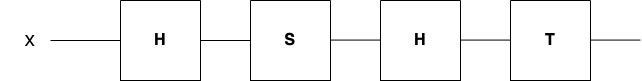
\includegraphics[width = 11cm]{./Images/circ2.png}
    \caption{}
    \label{fig1}
\end{figure}
\begin{definition}{Circuito}{}
    Definiamo come \textbf{circuito} un modello di computazione nella quale l'informazione
    è trasportata dai 'fili' (wires) attraverso una rete di 'porte' (gates), le quali rappresentano
    l'operazione applicata all'informazione trasportata.
\end{definition}
Nel modello quantistico, i fili e le porte rappresentano rispettivamente i qubits e le operazioni applicabili su di essi.
Ad esempio, la figura \ref{fig1} rappresenta l'applicazione delle operazioni $H$, $S$, $H$ e $T$ su un
singolo qubit. I circuiti quantistici hanno spesso i qubits inizializzati a $|0\rangle$. Se preferiamo,
è possibile rappresentare alla fine del circuito il nuovo stato a seguito delle trasformazioni, come mostrato
nella figura \ref{fig2}.

\begin{figure}[h]
    \centering
    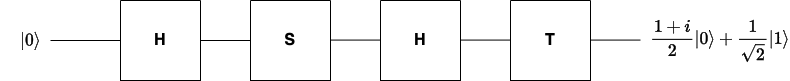
\includegraphics[width = 12cm]{./Images/circ3.png}
    \caption{}
    \label{fig2}
\end{figure}

La figura \ref{fig4}, invece, mostra un'operazione su un sistema multiplo, a due qubit. La prima,
intuitivamente, rappresenta l'operazione di Hadamard; la seconda, invece, è il controlled-NOT, dove il cerchio
riempito rappresente il qubit di controllo, mentre il $\otimes$ rappresenta il qubit target.

\begin{figure}[h]
    \centering
    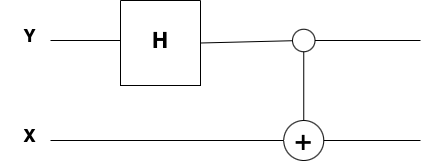
\includegraphics[width = 8cm]{./Images/circ42.png}
    \caption{}
    \label{fig4}
\end{figure}

Notiamo anche che nel modello è implicito l'applicazione dell'operazione identità sul qubit $X$. Sia quindi
$U$ la matrice unitaria rappresentante le due operazioni. $U$ è definita come:
\begin{equation*}
    U = \left(\mathbb{1} \otimes H \right)\left(|0\rangle\langle0| \otimes \mathbb{1} + |1\rangle\langle1| \otimes \phi_X\right) = 
    \left(\begin{array}{cccc}
        \frac{1}{\sqrt{2}} & \frac{1}{\sqrt{2}} & 0 & 0 \\ \\
       0 & 0 & \frac{1}{\sqrt{2}} & - \frac{1}{\sqrt{2}} \\ \\
       0 & 0 & \frac{1}{\sqrt{2}} & \frac{1}{\sqrt{2}} \\ \\
        \frac{1}{\sqrt{2}} & -\frac{1}{\sqrt{2}} & 0 & 0 
    \end{array}\right)
\end{equation*}

Abbiamo che:
\begin{equation*}
    \begin{array}{l}
        U|00\rangle = |\phi^+\rangle \\
        U|01\rangle = |\phi^-\rangle \\
        U|10\rangle = |\psi^+\rangle \\
        U|11\rangle = -|\psi^-\rangle \\
    \end{array}
\end{equation*}

I fili con due linee rappresentano i classici bit. Vengono utilizzati dopo aver eseguito una misurazione
come mostrato nella figura \ref{fig5}.

\begin{figure}[h]
    \centering
    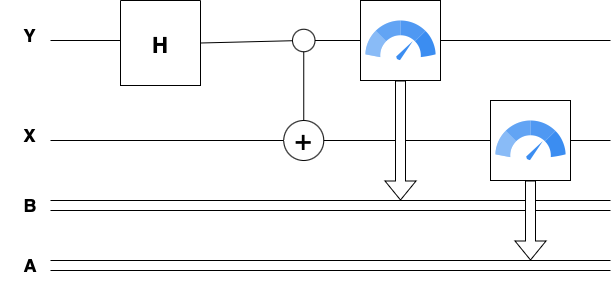
\includegraphics[width = 10cm]{./Images/MES.png}
    \caption{}
    \label{fig5}
\end{figure}

È spesso conveniente rappresentare i fili dei bit dopo la misurazione sullo stesso livello dei fili dei
qubit, come mostrato nella figura \ref{fig6}

\begin{figure}[h]
    \centering
    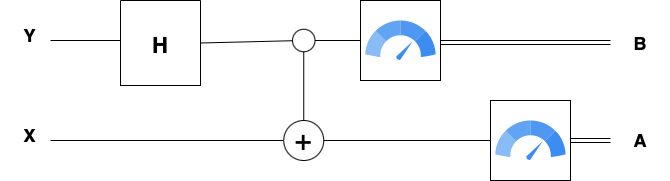
\includegraphics[width = 11cm]{./Images/mis.png}
    \caption{}
    \label{fig6}
\end{figure}

Ecco alcune porte comunemente usate per 1 o più qubit:

\begin{figure}[h]
    \centering
    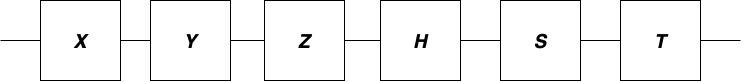
\includegraphics[width = 10cm]{./Images/Pauli.png}
    \caption{}
    \label{fig7}
\end{figure}

La figura \ref{fig7} rappresenta le operazioni che si fanno su un singolo qubit, abbiamo
in ordine: $\sigma_x$, $\sigma_y$, $\sigma_z$, Hadamard e le due Phase Operations.


La porta Not possiamo rappresentarla anche come nella figura \ref{fig8}.

\begin{figure}[h]
    \centering
    \begin{minipage}[b]{0.48\textwidth}
        \centering
        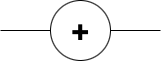
\includegraphics[width=\textwidth]{Images/plus.drawio.png}
        \caption{Not gate}
        \label{fig8}
    \end{minipage}
    \hspace{0.02\textwidth} % Spazio tra le immagini
    \begin{minipage}[b]{0.48\textwidth}
        \centering
        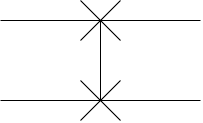
\includegraphics[width=\textwidth ]{Images/x.drawio.png}
        \caption{SWAP gate}
        \label{fig9}
    \end{minipage}
\end{figure}



\begin{figure}[h]
    \centering
    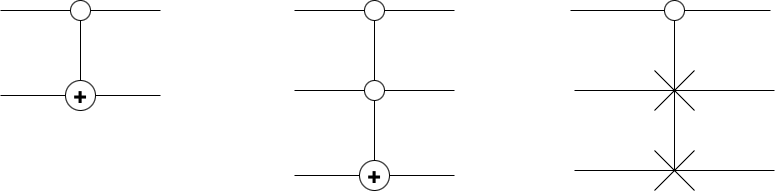
\includegraphics[width = 11cm]{./Images/LAST.drawio.png}
    \caption{}
    \label{fig10}
\end{figure}

\begin{figure}[h]
    \centering
    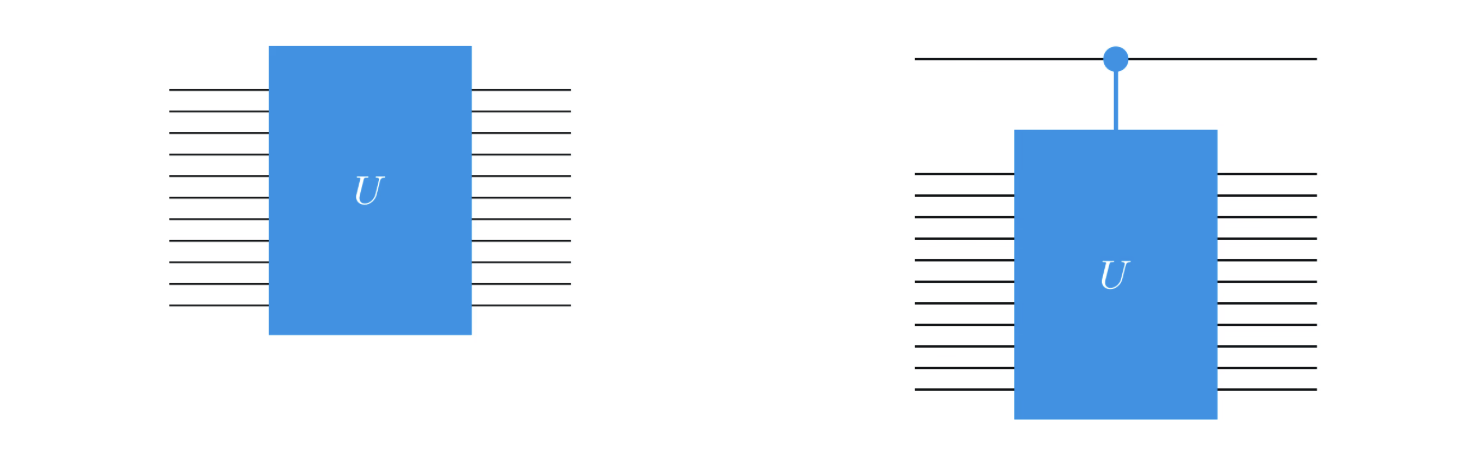
\includegraphics[width = 10cm]{./Images/ucontr.png}
    \caption{}
    \label{fig11}
\end{figure}

La figura \ref{fig9} rappresenta la porta SWAP. Infine la figura \ref{fig10} rappresentano le
porte di controllo, rispettivamente \textbf{controlled-NOT}, \textbf{controlled-controlled-NOT} e \textbf{controlled-SWAP}.

Operazioni arbitrarie sono rappresentate da rettangoli nominati con il nome dell'operazione unitaria.
La figura \ref{fig11} mostra un esempio. La figura a destra è la versione controllata.

\newpage
\subsection{Limitazioni nell'informazione quantistica}
\subsubsection{Irrillevanza della fase globale}
Siano $|\psi\rangle$ e $\phi\rangle$ due vettori unitari che rappresentano due stati 
quantistici. Assumiamo che esista un numero complesso $\alpha$, con $|\alpha| = 1$, tale che:
\begin{equation*}
    |\phi\rangle = \alpha |\psi\rangle
\end{equation*}
Allora diciamo che i vettori $|\phi\rangle$ e $|\psi\rangle$ \textbf{differiscono di una fase globale}.
Diciamo anche che $\alpha$ è la fase globale.

Consideriamo, quindi, un sistema che sta in uno dei due stati, $|\phi\rangle$ o $|\psi\rangle$
e che differiscono di una fase globale. Analizziamo cosa succede durante la misurazione. Nel caso
in cui il sistema si trovi nello stato $|\psi\rangle$, abbiamo che la probabilità di misurare
uno stato classico $a \in \Sigma$ è:
\begin{equation*}
    |\langle a|\psi\rangle|^2
\end{equation*}
Nel secondo caso, in cui lo stato sia $|\phi\rangle$, la probabilità che la misurazione dia come 
risultato lo stato $a \in \Sigma$ è:
\begin{equation*}
    |\langle a|\phi\rangle|^2 = |\alpha\langle a|\psi\rangle|^2 = |\alpha|^2 |\langle a|\psi\rangle|^2 = |\langle a|\psi\rangle|^2
\end{equation*}
perchè $|\alpha|^2 = 1$. Notiamo che la probabilità di misurare uno stato classico $a$ è esattamente lo stesso
per i due stati.

Consideriamo ora l'applicazione di un'operazione unitaria $U$ su entrambi gli stati. Nel caso
in cui lo stato iniziale è $|\psi\rangle$, allora dopo l'applicazione il nuovo stato diventa:
\begin{equation*}
    U|\psi\rangle
\end{equation*}
Nel caso, invece, in cui lo stato iniziale è $|\phi\rangle$, dopo l'applicazione lo stato diventa:
\begin{equation*}
    U|\phi\rangle = \alpha U|\psi\rangle
\end{equation*}
Notiamo che i due stati risultanti differiscono dalla stessa fase globale $\alpha$.

Concludiamo che, i due stati che differiscono da una fase globale sono completamente indistinguibili.
Per questo, $|\phi\rangle$ e $|\psi\rangle$ sono considerati \textbf{equivalenti}, e sono visti effettivamente
come lo stesso stato.
\begin{example}{}{}
    Ad esempio $|-\rangle$ e $-|-\rangle$ differiscono per la fase globale $-1$, quindi possono
    essere considerati lo stesso stato.
\end{example}
\subsubsection{Teorema no-cloning}
\begin{theorem}{No-cloning}{}
    Siano $X$ ed $Y$ due sistemi che condividono lo stesso insieme di stati classici $\Sigma$
    (avente almeno 2 elementi). Allora, possiamo affermare che \textbf{non} esiste uno stato 
    quanistico $|\phi\rangle$ di $Y$ e un'operazione unitaria $U$ sul sistema composto $(X,Y)$
    tale che
    \begin{equation*}
        U(|\psi\rangle \otimes |\phi\rangle) = |\psi\rangle \otimes |\psi\rangle \quad \forall |\psi\rangle \in X
    \end{equation*}    
\end{theorem}
\begin{proof}
    $\Sigma$ deve contenere almeno due elementi. Scegliamo, quindi, $a,b \in \Sigma$, con $a \not = b$.
    Supponiamo \textbf{per assurdo} che esista uno stato quantistico $|\phi\rangle$ e un'operazione unitaria $U$ sul sistema composto $(X,Y)$
    tale che
    \begin{equation*}
        U(|\psi\rangle \otimes |\phi\rangle) = |\psi\rangle \otimes |\psi\rangle \quad \forall |\psi\rangle \in X
    \end{equation*}
    Nel nostro caso:
    \begin{equation*}
        U(|a\rangle \otimes |\phi\rangle) = |a\rangle \otimes |a\rangle \wedge U(|b\rangle \otimes |\phi\rangle) = |b\rangle \otimes |b\rangle
    \end{equation*}
    Consideriamo il caso in cui $|\psi\rangle = \frac{1}{\sqrt{2}}|a\rangle + \frac{1}{\sqrt{2}}|b\rangle$.
    Sfruttando la caratteristica della linearità del prodotto tensoriale nel primo argomento ed
    la linearità del prodotto matrice-vettore nel secondo argomento, abbiamo che:
    \begin{equation*}
        \large
        \begin{array}{c}
            U\left(\left(\frac{1}{\sqrt{2}}|a\rangle + \frac{1}{\sqrt{2}}|b\rangle\right) \otimes |\phi\rangle \right) \\ \\
            = U\left(\frac{1}{\sqrt{2}}|a\rangle \otimes |\phi\rangle + \frac{1}{\sqrt{2}}|b\rangle \otimes |\phi\rangle\right) \\ \\
            = \frac{1}{\sqrt{2}}|a\rangle \otimes |a\rangle + \frac{1}{\sqrt{2}}|b\rangle \otimes |b\rangle
        \end{array}
    \end{equation*}
    Svolgendo i conti senza sfruttare la linearità degli argomenti, notiamo che:
    \begin{equation*}
        \begin{array}{c}
            U\left(\left(\frac{1}{\sqrt{2}}|a\rangle + \frac{1}{\sqrt{2}}|b\rangle\right) \otimes |\phi\rangle \right) \\ \\
            = \left(\frac{1}{\sqrt{2}}|a\rangle + \frac{1}{\sqrt{2}}|b\rangle\right) \otimes \left(\frac{1}{\sqrt{2}}|a\rangle + \frac{1}{\sqrt{2}}|b\rangle\right) \not = \frac{1}{\sqrt{2}}|a\rangle \otimes |a\rangle + \frac{1}{\sqrt{2}}|b\rangle \otimes |b\rangle
        \end{array}
    \end{equation*}
\end{proof}
\begin{oss}{}{}
    La \textbf{clonazione perfetta} non esiste, ma è possibile clonare con una percentuale di accuratezza
    limitata.
\end{oss}
\begin{oss}{}{}
    È possibile clonare perfettamente stati appartenenti a una base standard, come gli stati classici dei qubits.
\end{oss}

Costruiamo un circuito in grado di clonare uno stato classico del qubit, utilizzando l'operazione del
\textbf{control-not}:
\begin{figure}[h]
        \centering
        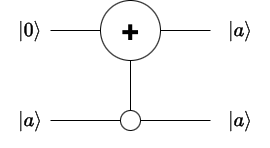
\includegraphics[width = 4cm]{./Images/example.png}
        \caption{}
\end{figure}

\subsection{Teletrasporto Quantistico}
\begin{definition}{Teletrasporto Quantistico}{}
    Definiamo come \textbf{teletrasporto quantistico} il protocollo tale che la sua funzione è il trasporto
    di informazione sfruttando gli e-bit (stati quantistici entangled).
\end{definition}
Siano, quindi, Alice (mittente) e Bob (destinatario) due entità che vogliono scambiarsi un qubit. Assumiamo
che entrambe le entità condividano un e-bit: Alice conserva il qubit \textbf{A} e Bob il qubit \textbf{B} e la
loro unione formano lo stato \textbf{entangled} $|\phi^+\rangle = \frac{1}{\sqrt{2}}|00\rangle + \frac{1}{\sqrt{2}}|11\rangle$.
Alice vuole 'spedire' il qubit \textbf{Q}, ovvero far in modo che Bob abbia un qubit avente lo stesso stato. 
Bob ed Alice non conoscono alcuna informazione riguardo allo stato Q. Non vi sono
assunzioni riguardo a quest'ultimo, quindi potrebbe essere anche uno stato entangled con un altro stato.

La figura \ref{fig12} mostra il circuito che descrive il funzionamento del protocollo.
\begin{figure}[h]
    \centering
    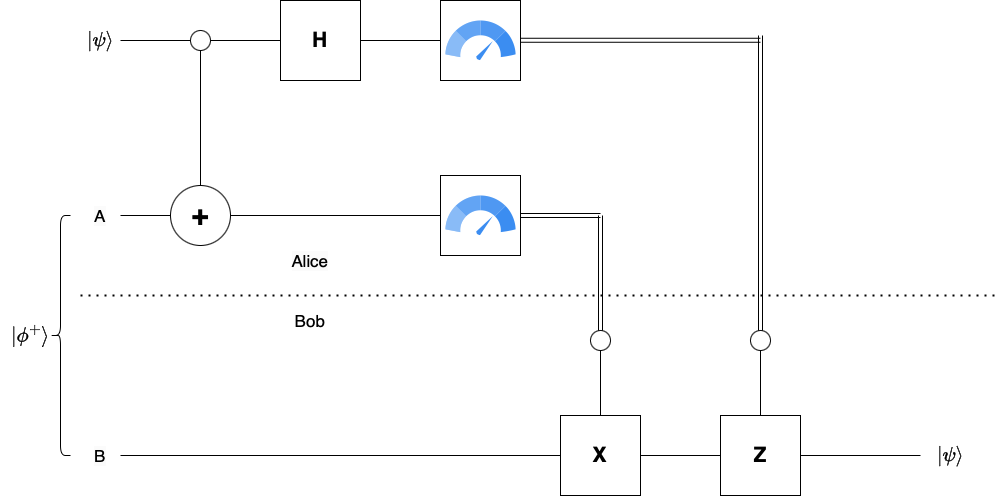
\includegraphics[width = 12.1cm]{./Images/telepng.png}
    \caption{}
    \label{fig12}
\end{figure}
\begin{oss}{}{}
    Notiamo che il qubit Q che Alice vuole trasmettere a Bob viene distrutto, richiamando
    quindi il teorema no-cloning. Questo è il costo del teletrasporto quantistico.
\end{oss}

Andiamo ora ad analizzare il funzionamento del circuito. Sia Q nello stato generico 
\begin{equation*}
    \alpha |0\rangle + \beta |1\rangle
\end{equation*}
Sia (B,A,Q) il sistema che dello stato del circuito. Lo stato iniziale di tale sistema è:
\begin{equation*}
    |\phi^+\rangle \otimes \left(\alpha |0\rangle + \beta |1\rangle\right) = \frac{1}{\sqrt{2}} \left(\alpha|000\rangle + \alpha|110\rangle + \beta|001\rangle + \beta|111\rangle\right)
\end{equation*}
Lo stato dopo aver applicato l'operazione controlled-not diventa:
\begin{equation*}
    \frac{1}{\sqrt{2}} \left(\alpha|000\rangle + \alpha|110\rangle + \beta|011\rangle + \beta|101\rangle\right)
\end{equation*}
Applichiamo ora l'operazione di Hadamard, trasformando lo stato in:
\begin{equation*}
    \begin{array}{c}
        \frac{1}{\sqrt{2}} \left(\alpha|00\rangle|+\rangle + \alpha|11\rangle|+\rangle + \beta|01\rangle|-\rangle + \beta|10\rangle|-\rangle\right) \\ \\ 
        = \frac{1}{2} \left(\alpha|000\rangle + \alpha|001\rangle + \alpha|110\rangle +  \alpha|111\rangle + \beta|010\rangle - \beta|011\rangle + \beta|100\rangle - \beta|101\rangle\right) \\ \\
        = \frac{1}{2}\left(\alpha |0\rangle + \beta |1\rangle\right)|00\rangle + \frac{1}{2}\left(\alpha |0\rangle - \beta |1\rangle\right)|01\rangle + \frac{1}{2}\left(\alpha |1\rangle + \beta |0\rangle\right)|10\rangle + \frac{1}{2}\left(\alpha |1\rangle - \beta |0\rangle\right)|11\rangle 
    \end{array}
\end{equation*}
Analizziamo i possibili casi di misurazione:
\begin{itemize}
    \item La probabilità di misurare $A = 0$ e $Q = 0$ è di
            \begin{equation*}
                \Vert \frac{1}{2}\left(\alpha |0\rangle + \beta |1\rangle\right)|00\rangle \Vert^2 = \frac{1}{4}\left(|\alpha|^2 + |\beta|^2\right) = \frac{1}{4}
            \end{equation*}
        e lo stato $(B,A,Q)$ diventa:
        \begin{equation*}
            \left(\alpha |0\rangle + \beta |1\rangle\right)|00\rangle
        \end{equation*}
        In questo caso, Bob non deve applicare alcuna operazione.
    \item La probabilità di misurare $A = 0$ e $Q = 1$ è di
    \begin{equation*}
        \Vert \frac{1}{2}\left(\alpha |0\rangle - \beta |1\rangle\right)|01\rangle \Vert^2 = \frac{1}{4}\left(|\alpha|^2 - |\beta|^2\right) = \frac{1}{4}
    \end{equation*}
    e lo stato $(B,A,Q)$ diventa:
    \begin{equation*}
        \left(\alpha |0\rangle - \beta |1\rangle\right)|01\rangle
    \end{equation*}
    In questo caso, Bob deve applicare l'operazione $Z$ al suo qubit $B$, ovvero:
    \begin{equation*}
        \left(\alpha |0\rangle + \beta |1\rangle\right)|01\rangle
    \end{equation*}
    \item La probabilità di misurare $A = 1$ e $Q = 0$ è di
        \begin{equation*}
            \Vert \frac{1}{2}\left(\alpha |1\rangle + \beta |0\rangle\right)|10\rangle \Vert^2 = \frac{1}{4}\left(|\alpha|^2 + |\beta|^2\right) = \frac{1}{4}
        \end{equation*}
        e lo stato $(B,A,Q)$ diventa:
        \begin{equation*}
            \left(\alpha |1\rangle + \beta |0\rangle\right)|10\rangle
        \end{equation*}
        In questo caso, Bob deve applicare l'operazione $X$ al suo qubit $B$, ovvero:
        \begin{equation*}
            \left(\alpha |0\rangle + \beta |1\rangle\right)|10\rangle
        \end{equation*}
    \item La probabilità di misurare $A = 1$ e $Q = 1$ è di
    \begin{equation*}
        \Vert \frac{1}{2}\left(\alpha |1\rangle - \beta |0\rangle\right)|11\rangle \Vert^2 = \frac{1}{4}\left(|\alpha|^2 + |\beta|^2\right) = \frac{1}{4}
    \end{equation*}
    e lo stato $(B,A,Q)$ diventa:
    \begin{equation*}
        \left(\alpha |1\rangle - \beta |0\rangle\right)|11\rangle
    \end{equation*}
    In questo caso, Bob deve applicare l'operazione $X$ e $Z$ al suo qubit $B$, ovvero:
    \begin{equation*}
        \left(\alpha |0\rangle + \beta |1\rangle\right)|11\rangle
    \end{equation*}
\end{itemize}
Osserviamo che in tutti i casi, lo stato di $B$ è uguale a $\alpha |0\rangle + \beta |1\rangle$, ovvero
lo stato iniziale di $Q$; abbiamo, quindi, teletrasportato l'informazione del qubit $Q$ da Alice
a Bob.
    \section{Fondamenta degli Algoritmi Quantistici}
In questa sezione viene descritto quali sono e come vengono eseguite
le computazioni su un computer quantistico. Inizialmente vengono analizzate
le differenze che si hanno quando ci si confronta con un modello di computazione classico
e, nello specifico, verranno elencati algoritmi quantistici che offrono
vantaggi rispetto ad una computazione classica.
\subsection{Computazione classica vs Computazione quantistica}
Uno dei primi vantaggi che una computazione quantistica può offrire
è sicuramente quello del \textbf{tempo}; infatti, per alcuni problemi, sono state proposte
nuove soluzione che hanno dimostrato un incremento esponenziale del tempo di esecuzione.

Mediante l'utilizzo di porta logica di \textbf{Toffoli}, è possibile simulare circuiti 
logici classici su circuiti quantistici. La porta di \textbf{Toffoli} riesce
ad implementare un qualsiasi circuto Booleano; inoltre, la reversibilità di tale porta,
contribuisce alla simulazione dei circuiti classici su circuiti quantistici.

Ad esempio, riusciamo a simulare la porta NAND (irreversibile) con la porta di Toffoli.
La figura \ref{fig13} mostra il NAND implementato con il Toffoli gate.
\begin{figure}[h]
    \centering
    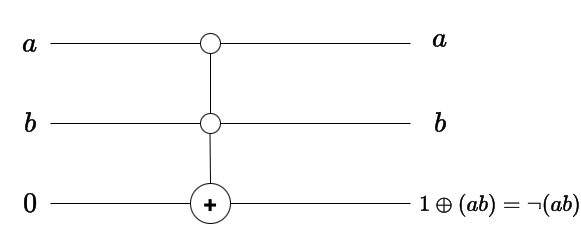
\includegraphics[width = 7cm]{./Images/toff.png}
    \caption{}
    \label{fig13}
\end{figure}

\begin{fact}{}{}
    È possibile implementare qualsiasi circuito booleano classico attraverso la porta di Toffoli.
\end{fact}

\subsection{Parallelismo Quantistico}
Data una funzione $f(x)$, definiamo (a parole semplici) il \textbf{parallelismo
quantistico} come una caratteristica del mondo quantistico che permette
la valutazione di $f(x)$ per diversi valori di $x$ simultaneamente.

Supponiamo che $f(x): \{0,1\} \rightarrow \{0,1\}$. Calcolare tale funzione
in un'ambiente quantistico necessita la definizione di un'operazione 
unitaria, solitamente chiamata $U_f$, rappresentata nella figura \ref{fig14}.
\begin{figure}[h]
    \centering
    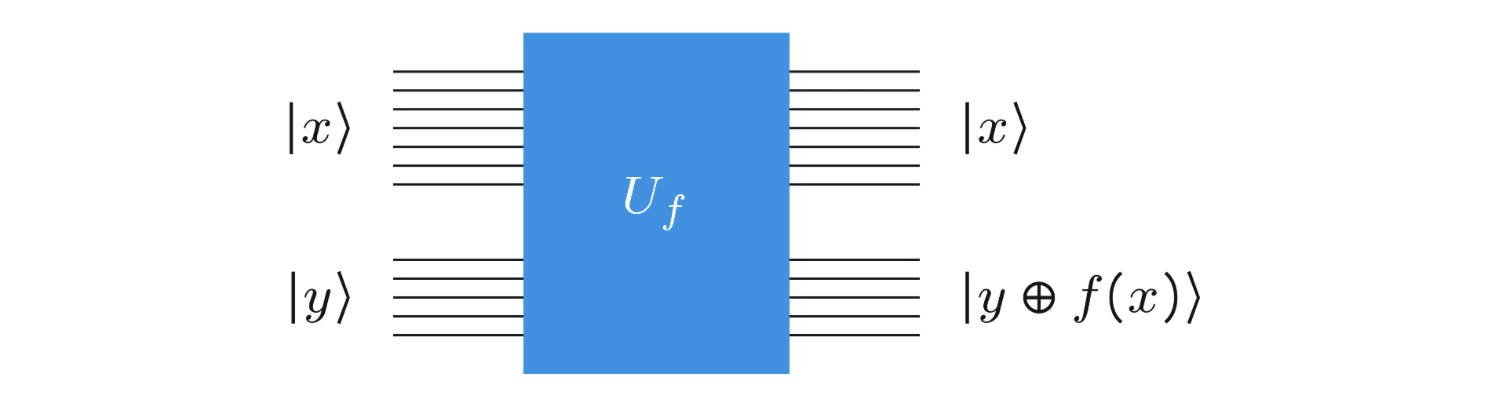
\includegraphics[width = 10cm]{./Images/uf.png}
    \caption{}
    \label{fig14}
\end{figure}
 Quindi dobbiamo considerare un computer quantistico a due qubit,
 che inizializza lo stato a $|x,y\rangle$. 
 
 Dopo l'applicazione di $U_f$, riusciamo a trasformare lo stato in $|x,y \oplus f(x)\rangle$, 
 dove $\oplus$ indica l'operazione \textit{bitwise} dello XOR. Denominiamo il primo registro come
 \textit{data} e il secondo come \textit{target}.

 \begin{oss}{}{}
    Se $y=0$, allora lo stato finale del secondo qubit è equivalente
    ad $f(x)$.
 \end{oss}

 Supponiamo ora che inizializziamo il registro \textit{data} nella superposizione
 \begin{equation*}
    |+\rangle = \frac{1}{\sqrt{2}}|0\rangle + \frac{1}{\sqrt{2}}|1\rangle
 \end{equation*}
 la quale può essere ottenuta, ad esempio, applicando la porta di Hadamard
 sullo stato base $|0\rangle$. Supponiamo anche di inizializzare il ragistro
 \textit{target} con $|0\rangle$. Quindi:
 \begin{equation*}
    \begin{array}{c}
        U_f\left(\left(\frac{1}{\sqrt{2}}|0\rangle + \frac{1}{\sqrt{2}}|1\rangle\right)\otimes |0\rangle\right) = \frac{1}{\sqrt{2}}\left(U_f \left(|0\rangle \otimes |0\rangle\right) + U_f \left(|1\rangle \otimes |0\rangle\right)\right) \\ \\
        = \frac{1}{\sqrt{2}}\left(|0\rangle \otimes |f(0)\rangle + (|1\rangle \otimes |f(1)\rangle)\right)
    \end{array}
 \end{equation*}
 Osserviamo, incredibilmente, di come ci sia bastata una singola 
 valutazione per computare la funzione su tutto il dominio della funzione ($\{0,1\}$).
 Abbiamo semplicemente sfruttato l'abilità di un qubit di stare
 in una superposizione tra stati differenti.

 Questa procedura è generalizzabile per tutte le funzioni aventi
 un numero arbitrario di bits, utilizzando un'operazione
 generale conosciuta come \textbf{trasformazione di Hadamard}, o anche
 \textbf{trasformazione di Walsh-Hadamard}. È semplicemente l'applicazione 
 di $n$ porte di Hadamard in parallelo su $n$ qubits.
 \begin{example}{}{}
    Ad esempio, per $2$ qubit inizializzati allo stato base $|0\rangle$,
    la trasformazione ci da come output:
    \begin{equation*}
        \left(\frac{|0\rangle + |1\rangle}{\sqrt{2}}\right)\left(\frac{|0\rangle + |1\rangle}{2}\right) = \frac{|00\rangle + |01\rangle +|10\rangle +|11\rangle}{\sqrt{2}}
    \end{equation*}
 \end{example}
 Nel esempio, denotiamo con $H^{\otimes 2}$ l'operazione parallela delle porte di Hadamard. Più in generale, 
 la computazione di tale trasformazione su $n$ qubit con stato di partenza a $|0\rangle$ è equivalente a
 \begin{equation*}
    \frac{1}{\sqrt{2^n}}\sum_{x \in \Sigma} |x\rangle
 \end{equation*}
ed indichiamo con $H^{\otimes n}$ tale operazione. Otteniamo una superposizione di
\textbf{$2^n$} stati usando solo \textbf{$n$} porte.

La misurazione dello stato $\frac{1}{\sqrt{2^n}}\sum_{x \in \Sigma} |x\rangle$ ci restituisce solo $f(x)$, per un singolo
valore $x$. Non ci è tanto utile, quindi è necessaria l'abilità di estrazione di informazioni
su più di un valore di $f(x)$ dalla superposizione per poter sfruttare questo parallelismo.

\subsection{Algoritmo di Deutsch}
		
\end{document}